%% using aastex version 6


\newcommand{\opsfp}{N$_{FP_{obs}}$}
\newcommand{\opspc}{N$_{PC_{obs}}$}
\newcommand{\opsN}{N$_{obs}$}
\newcommand{\trueopspc}{T$_{PC_{obs}}$}
\newcommand{\missedfp}{T$_{FP_{obs}}$ - N$_{FP_{obs}}$}
\newcommand{\invfp}{N$_{FP_{inv}}$}
\newcommand{\invpc}{N$_{PC_{inv}}$}
\newcommand{\invN}{N$_{inv}$}
\newcommand{\sfatce}{SFA-TCE}


\subsection{Calculating Completeness and Reliability}
We use the \injtce\, \scrtce\ and \invtce\ data sets to determine how effective the Robovetter, \S\ref{s:robovetter}, is at identifying false alarms while not removing true transits. Ultimately we would like a measure of the Robovetter completeness, the fraction of true transits that are created into PCs, and the Robovetter reliability, the fraction of PCs that are truly PCs.   Completeness is easily measured by simply measuring the fraction of on-target \injtce s that are turned PCs. In the next section we will describe how we calculate reliability using a set of simulated false alarms.

\subsubsection{Derivation of Reliability}
\label{s:relcalc}
To assess the catalog reliability, we will assume that the \scrtce s and \invtce s are similar to those we see in the \opstce\ set. Close visual inspection of many in the sample validates that assumption.  One way to calculate the reliability of the catalog from our false alarm sets is to first calculate our effectiveness at correctly identifying a known false alarm as such.  Then given the number of false alarms we identify in the \opstce\ set, we can determine the reliability of the catalog against the type of false alarms present in the the simulated sets (\invtce\ and \scrtce). This method assumes the frequency of the different types of false alarms is well emulated by the simulated data sets. 



Effectiveness ($E$) is defined as the fraction of false positives correctly identified as false positives in the \opstce\ data set. 
\begin{equation}
\label{effect1}
E \equiv \frac{N_{FP_{obs}}}{T_{FP_{obs}}}
\end{equation}
Notice we are using N to indicate a measurable number, and T to indicate the ''True" number, assuming $E\leq 1 $.  If the simulated false alarm TCEs (e.g. \invtce) accurately reflects the \opstce\ false positives, $E$ can be calculated as the number of simulated false alarm TCEs identified as false positives (\invfp) divided by the number of inverted TCEs (\invN). 

\begin{equation}
\label{effect2}
E = \frac{N_{FP_{inv}}}{N_{inv}}
\end{equation}

Reliability, $R$, is defined as the ratio of the true observed PCs,\trueopspc, to the total number of observed PCs,\opspc. At this point we can drop the \textit{obs} and \textit{inv} designation as all the inversion values are wrapped up in $E$, and the $N$ values shown below refer entirely to the number of candidates (PC) or false positives (FP) determined to be the \opstce set so that $N=N_{PC} + N_{FP}$. From the definition for reliability, we rewrite in terms of the number of true false positives.

\begin{equation}
R \equiv \frac{T_{PC}}{N_{PC}} =  1 + \frac{T_{PC}-N_{PC}}{N_{PC}} 
= 1 + \frac{N_{ops} - T_{FP} - N_{PC}}{N_{PC}}
\end{equation}
Substitute $N_{FP}=N-N_{PC}$ and you get another useful way to think about reliability, as the number of unidentified false positives relative to the number of candidates.

\begin{equation}
\label{rel}
R = 1 - \frac{T_{FP}-N_{FP}}{N_{PC}}
\end{equation}

However, the true number of observed FPs is not known. Using the effectiveness value measured from inversion (or scrambling) (equation \ref{effect2}) and combining it with our definition for effectiveness (equation \ref{effect2}), we get (T$_{FP}$):
\begin{equation}
T_{FP} = \frac{N_{FP}}{E} 
\end{equation}

Substituting into equation \ref{rel},
\textbf{
\begin{equation}
R= 1 - \frac{N_{FP}}{N_{PC}}(\frac{1-E}{E})
\end{equation}
}.

%or, in terms of the unreliability ($U= 1-R$) and the Ineffectiveness ($I=1-E$)
%\begin{equation}
%U=\frac{N_{FP}}{N_{PC}}(\frac{I}{E})
%\end{equation}

%\subsubsection{Example}

%If you choose one MES/Period bin, you can use the inversion effectiveness to calculate the reliability of the catalog for this bin. We show one example of the robovetter run below. If we consider the MES range of 10-20 and the Period range of 10-200 days, we find that the robovetter has $E=97.7\%$. The number of false positives in that bin is 2613 and the number of PCs is 730.  Thus the reliability is $1 - \frac{2613}{730} \times \frac{1-.977}{.977} = 91.7\% $.  This means that of the 730 reported PCs, 60 are actually false positives.

If the number of observed false positives is much larger than the number of false positives identified in the inversion run, it is possible to get a negative reliability. This likely means that we do not have a good measure of the effectiveness.  Given the number of observed false positives, we should have found more planet candidates than we did. Or, given the measure of the effectiveness we have, the number of FPs that were missed is greater than the number of PCs that we have left to draw from.  This can happen if the effectiveness measured by inversion is lower than the true value. For example, if the number of hard-to-identify false alarms is larger in the \invtce\ data set than in the \opstce\ data set.   

\subsection{Verifying Assumptions}
In order to use the \scrtce\ and \invtce\ sets to determine the reliability of our catalog we must first verify that the properties of these simulated false positives are similar to those of the false positive in the \opstce\ set.  The intent of these simulated data sets is to emulate the false positives that create not-transit-like \opstce s.  There are many different reasons a false positive will fit in this category. The method for measuring reliability that we outline above hinges on the assumption that for any part of parameter space the fraction of false alarms caused by a particular type of false positive is the same between the simulated and observed data sets.  It is for this reason that we removed the TCEs caused by KOIs and EBs in the simulated data sets, see \S\ref{s:clean}. Since inverted EBs are not the type of false positive we are trying to evaluate for reliability, we did not want to include them in our sample.

Figure\,\ref{f:tces} demonstrates that the number of TCEs from inversion and scrambling individually is smaller than the number of false positives in the \opstce\ set. This is in part do to the fact that by removing the stars that contain EBs and KOIs we are searching a significantly smaller number of stars. 

The different metrics used by the Robovetter provides one way to evaluate how well the simulated data sets emulate the \opstce s.  Each metric measures some aspect of the TCE. For instance LPP measures whether the folded and binned light curve is transit shaped, and Skye measures whether the individual transits are likely due to rolling band.  If the simulated TCEs can be used to measure reliability in the way described above, then the the fraction of false alarms in any period bin caused by any particular metric should match between the two sets.  In Figures~\ref{f:fractionFailMetric} and \ref{f:fractionFilMetricMes} we show that this is basically true for both \invtce s and \scrtce s, especially for periods longer than 100 days and MES less than 15 (the parameter space where the measure of reliability is most important).  Keep in mind that more than one metric can fail any particular TCE, so the total fraction of TCEs when added up across all metrics will be greater than one.  The 15 per cent differences seen for the LPP metric in the \invtce set are the largest variation we see in the period range and should be considered when one attempts to compute realistic error bars on the reliability measurements. 

For this paper which we attempt to provide an estimate of the reliability, we are satisfied with this basic agreement. For this paper we have decided to calculate the catalog reliability using a union of the \scrtce\ and \invtce\ set after they have been cleaned as described in \S\ref{s:clean}.  This decision is primarily driven by the fact that a larger set of simulated false alarms improves the precision of our reliability estimate.  And, this analysis shows that neither set is preferred across all of parameter space. However, both \scrtce\ and \invtce\ sets and their Robovetter dispositions are available at the NASA Exoplanet Archive, and users may chose a different set of simulated false alarms to improve upon this estimate.  

\begin{figure*}
    \centering
    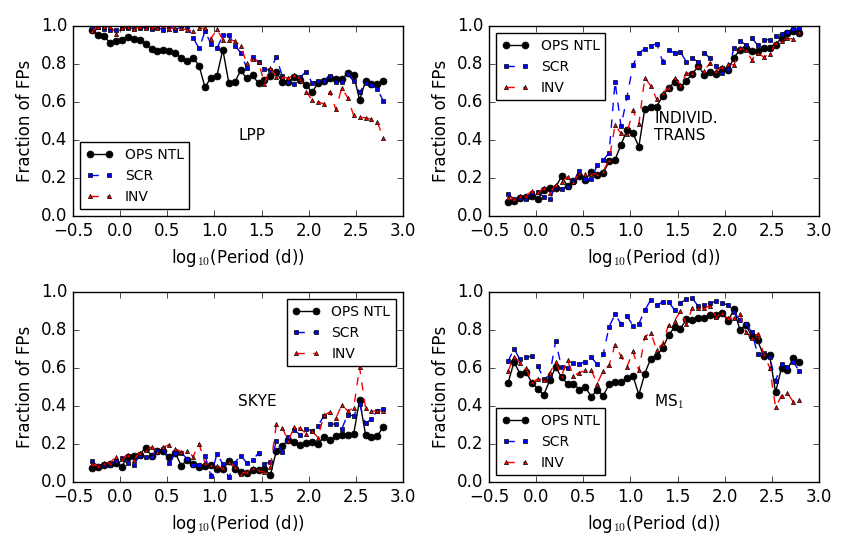
\includegraphics[width=0.9\linewidth]{fig-fractionFailsByMetric.png}
    \caption{The fraction of false positives failed by a particular type of Robovetter metric plotted against the logarithm of the period.  The fraction is plotted for not-transit-like FPs from the \opstce\ set in black, the \scrtce\ set in blue and the \invtce\ set in red. For each metric we include fails from either detrender (DV or Alt) for the metric stated in the middle of the plot. Upper left: LPP metric failures. Upper Right: TCEs that fails after removing a single transit due to any of the individual transit metrics.  Lower left: TCEs that fail after removing a single transit due to the Skye metric. Lower right: Model Shift 1 metric failures. }
    \label{f:fractionFailMetric}
\end{figure*}

\begin{figure*}
    \centering
    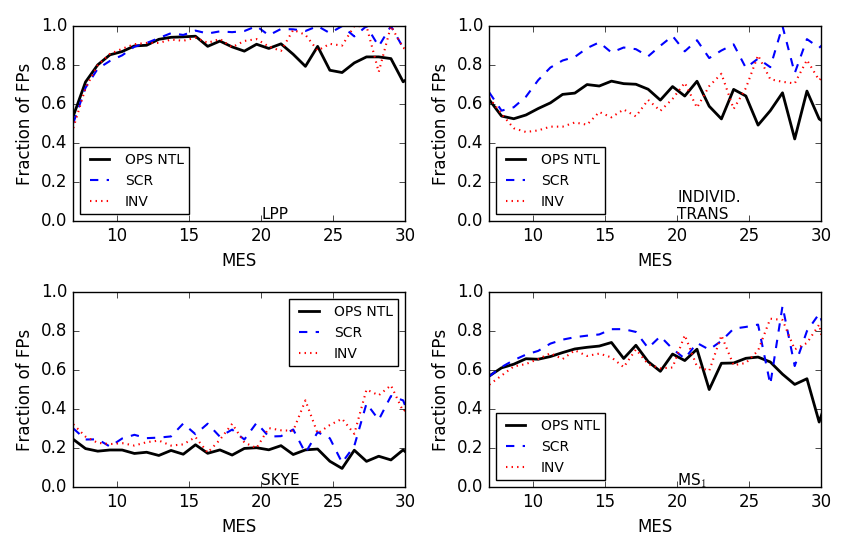
\includegraphics[width=0.9\linewidth]{fig-fractionFailsByMetricMes.png}
    \caption{The fraction of false positives failed by a particular type of Robovetter metric plotted against MES.  The fraction is plotted for not-transit-like FPs from the \opstce\ set in black, the \scrtce\ set in blue and the \invtce\ set in red. For each metric we include fails from either detrender (DV or Alt) for the metric stated in the middle of the plot. Upper left: LPP metric failures. Upper Right: TCEs that fails after removing a single transit due to any of the individual transit metrics.  Lower left: TCEs that fail after removing a single transit due to the Skye metric. Lower right: Model Shift 1 metric failures. }
    \label{f:fractionFailMetricMes}
\end{figure*}